\documentclass[11pt]{amsart}
\usepackage{hyperref}
\usepackage{cleveref}
\usepackage{color}
\usepackage{tikz}
\usepackage{times}
\usepackage[margin = 1in]{geometry}
\renewcommand{\i}[0]{{\bf i}}
\newcommand{\Emph}[1]{\textbf{\emph{#1}}}
\title{Research Statement}
\date{\today}
\author{Sylvester W. Zhang}
\date{\today}
\thanks{URL: \href{https://sylvesterzhang.com}{sylvesterzhang.com} Email:\href{mailto:swzhang@umn.edu}{swzhang@umn.edu}}
\begin{document}
\maketitle
I work on \Emph{algebraic combinatorics}, which is an area of research that often involves using abstract algebra to solve combinatorial problems, and conversely, using techniques from discrete mathematics (combinatorics) to answer algebraic questions. 

As the Fields medalist Timothy Gowers \cite{gowers2000two} noted, there are two cultures of mathematics, one focuses on \emph{problem-solving} while the other emphasizes \emph{theory-building}.
On the first side we have \Emph{combinatorics}, which studies discrete objects (e.g. permutations, graphs, integers, networks, algorithms, etc.) with a primary focus on enumeration (counting). It often emphasizes problem-solving techniques (tricks) over abstractions. In fact, many elegant combinatorial proofs, despite being extremely technical, are elementary enough to be understood by high school students. %As a rather young subject of study, only in the late 20th century did combinatorics become an independent branch of mathematics on its own right, because of its applications in various other areas of maths and physics, and more importantly, its connections to computer science and information theory.
Combinatorics has found many applications since the prosperity of computer sciences. For example, the navigation systems we use everyday, finding the best route between two points, can be naturally translated to a graph theory problem. And how efficient the navigation algorithm performs heavily depends on the combinatorial theory behind. Moreover, many other subjects like social networks, sorting and ranking algorithms, are all combinatorial problems in their essences.
However, despite being appreciated for having fruitful real-world applications in computer science and optimization theory, combinatorics is often criticized by many main stream mathematicians for ``having very little structure and consists of nothing but a large
number of problems." (\cite{gowers2000two}, p. 9)
On the other side, \Emph{abstract algebra} is the study of symmetries and algebraic structures (such as vector fields, groups, algebras, etc.), which are often highly abstract and theorized. Although being regarded as part of the ``central core" of mathematics, abstract algebra, along with many other so-called ``pure mathematics'', have always been accused to be useless in real world scenarios and consist of noting but abstract theories.

\Emph{Algebraic Combinatorics} is a young field of mathematics, born roughly in the 1970's, which is the magical combination of these two seemingly completely unrelated fields. %Only since the 1970's have algebraic combinatorics become an independent and respected area of study on its own right.
Almost miraculously, many algebraic structures can be interpreted in terms of simple (and often pretty) diagrams or graphs, which then allows us to tackle those abstract algebraic questions using concrete techniques from discrete mathematics. Just as Sara Billey said, ``Combinatorics is the nanotechnology of mathematics". On the other hand, abstract algebra has also proved to be very helpful in various kinds of problems in discrete mathematics which otherwise could be very technical and hard to solve. For example, in one of my undergraduate research projects on finding spanning trees in certain networks \cite{arb}, we struggled and failed to come up with an elementry proof, but the problem got resolved immediately once we incorporated certain ideas from abstract group theory (specifically, Galois theory). 
%

I found myself fascinated by these kinds of connections, and am always excited about the discovery of new connections during my research.
In particular, my research interests often lie in the crossroad of algebra, combinatorics, and statistical physics. Specifically, I am interested the following topics: cluster algebras, affine combinatorics, and integrable models in statistical physics, of which I will elaborate on the first two in this statement. The plan of this statement is as follows. In the first section, I will talk about my previous major contributions, which is in the area of \Emph{cluster algebras}. And in the second section, I will discuss my current main focuses, which is my thesis research project on \Emph{affine combinatorics} including several future directions.%, and \Emph{using integrable models to study special functions}.


\section{Cluster Algebras}
Cluster 	algebras are special kinds of commutative algebras. Loosely speaking, a \emph{cluster algebra} is a collection of Laurent polynomials (i.e. a polynomial divided by a monomial, e.g. $ab+cd+ef\over ace$), which is defined recursively and has vert nice combinatorial properties. They were first introduced by Fomin and Zelevinsky in 2002 as an algebraic framework for canonical basis of quantum groups, but have been found to be connected to many other areas in mathematics (e.g. hyperbolic geometry, homological algebra, plane curve singularity, etc.) and physics (thermodynamic Bethe Ansatz, Feynman integrals, $\mathcal{N}=4$ Yang-Mills, string theory, etc.) 

Among my several research interests, cluster algebra is the topic where I spent most of my time on. My main contribution in this are is a generalization of cluster algebras called \Emph{supersymmetric cluster algebras}.
%In particular, I worked on two generalizations of cluster algebras, one is \emph{supersymmetric cluster algebras} and another is called LP algebras.

%\subsection{Supersymmetric Cluster Algebras}

\subsection*{Background on Supersymmetric Cluster Algebras}
In particle physics, supersymmetry (SUSY) is a simple principle proposing a relationship between two kinds of basic particles, bosons and fermions. It appeared last century as an effort to unifying all physics theories. The mathematical framework for SUSY is a new kind of numbers called \emph{Grassmann numbers} or simply ``super numbers''. These numbers are defined in a similar spirit as complex numbers $a+b\i$ where $a,b$ are usual real numbers and $\i$ satisfy the relation $\i^2=-1$. Grassmann numbers looks like $a+b\theta_1+c\theta_2+d\theta_3+\cdots +e\theta_1\theta_2+f\theta_1\theta_3\cdots$, where $a,b,c,\cdots$ are usual numbers and $\theta_1,\theta_2,\cdots$ are new variables\footnote{Think of the $\theta_1,\theta_2,\cdots$ as the $\i$ in complex numbers, but this time we have many of them instead of just one.} which satisfy the relation $\theta_i\theta_j=-\theta_j\theta_i$ (anti-commutativity). Under this framework, the usual numbers ($a,b,c,\cdots$) correspond to bosons and the anti-commutative variables $\theta_i$'s correspond to fermions.

In recent years, a lot of progress have been made on extending the current theory of cluster algebras to a supersymmetric version (naively speaking, adding anti-commutative variables to cluster algebras), such as \cite{ovsienko2018cluster, shemyakova2022super} to name a few.
This line of research is not only a natural mathematical question to pursue, but also has  found application in theoretical physics \cite{gates2021cluster}.
\subsection*{My contribution}
In a serious of joint works with G. Musiker and N. Ovenhouse \cite{moz1,moz2,moz3}, we took the first step of understanding supersymmetric cluster algebras through a geometric lens. In particular, we introduced the notion of \Emph{super cluster algebras of geometric type}, motivated by Penner-Zeitlin's work on super-geometry \cite{penner2019decorated}. Our works generalize the notion of (classical) cluster algebras of geometric type, which is a canonical and motivating example in the theory of cluster algebras. 

In \cite{moz1,moz2}, we proved that, elements of a super cluster algebra (of geometric type) %(which are Laurent polynomials now involving anti-commutative variables) 
can be interpreted using \Emph{double dimer configurations}, a statistical-physics model first used to describe crystal structures of certain molecules. In the recent paper \cite{moz3}, we took a more algebraic approach and relate the combinatorics of double dimer models from super cluster algebras to the ortho-symplectic super-group $\textup{OSp}(1|2)$\footnote{$\textup{OSp}(1|2)$ is an abstract group of $3\times 3$ matrices whose entries are ``super numbers'', which is of fundamental importance in the algebraic theory of supersymmetry.}.
\subsection*{Future Directions}There are several future directions that my collaborators and I are planning to pursue.
\begin{enumerate}
	%\item Our works also suggest possible new mathematical objects which fit under the physical framework of SUSY. For example, as a byproduct, we found a super-number generalization of Fibonacci numbers. We believe that more meaningful supersymmetric combinatorics are yet to be discovered under this line of research.
	\item We plan to investigate the mathematical meanings of the statistical physics models (the double dimer models) which show up in our work. It is known that single dimer models are related to continued fractions. In a current joint work-in-progress with G. Musiker, N. Ovenhouse, and R. Schiffler, we are working on a generalization of this correspondence which suggests a higher-dimensional analogue of continued fractions.
	\item Our works on super cluster algebras of geometric type only provide an special class of super cluster algebras, despite being an important one. A more general, axiomatic theory of super cluster algebras is still out of reach. However, our works shed an light on this darkness since we provided the very first explicit formulae. We hope to continue in this direction and make further progress on a more general theory.
\end{enumerate}
\subsection*{Another Related Project}
I've also worked on a closely related project involving \Emph{Laurent Phenomenon (LP) Algebras}, which is another generalization of cluster algebras.
In cluster theory, one of the most important achievements is the proof of the positivity conjecture \cite{lee2015positivity}, which states that all elements of a cluster algebras only have positive coefficients\footnote{In other words, you will only see `+' signs in them.}. 

The same positivity property was conjectured for LP algebras as well, which has been wildly open. In the collaboration with E. Banaian, S. Chepuri, and E. Kelley \cite{bckz1}, we made the first progress on proving this conjecture in a special case. In a subsequent work (in-progress) \cite{bckz2}, we took the dimer-model approach and strengthened our previous result to all acyclic graph LP algebras, with only small restrictions on the chosen element.
%In , we focused on certain \Emph{acyclic-graph LP algebras} which are encoded by a tree-graph (a graph with no cycle), and proved that for a special class of such LP algebras, the positivity conjecture holds. 
%In a subsequent work (in-progress) \cite{bckz2}, we took the dimer-model approach and showed that those LP algebra elements can be interpreted using what we called the \Emph{higher mixed dimer configurations}. In this new approach, we strengthened our previous result to all acyclic graph LP algebras, with only small restrictions on the chosen element.

%
%In the future, I plan to continue working in this direction. 
%In fact, in a current joint work-in-progress with G. Musiker, N. Ovenhouse, and R. Schiffler, we are studying the combinatorics of the above mentioned double dimer models as well as generalized higher dimer models. In particular, we are investigating the number-theoretic consequences of these statistical physics models, which we hope to connect to some higher-dimensional analogues of continued fractions.

%\subsection{Laurent Phenomenon Algebras} Introduced by Lam and Pylyavskyy \cite{lam2012laurent}, Laurent Phenomenon (LP) algebras are generalizations of cluster algebras. LP algebras are related to \emph{electrical Lie algebras} which are certain algebraic models of electrical networks, and also, many other important generalizations of cluster algebras (such as Chekov-Shapiro algebras) are special cases of LP algebras.
%
%In cluster theory, one of the most important achievements is the proof of the positivity conjecture \cite{lee2015positivity}, which states that all elements of a cluster algebras are Laurent polynomials\footnote{A Laurent polynomial is a polynomial divided by a monomial, e.g. ${ab+cd-efg+d\over{ace}}$.} with only plus signs ($+$) in it. 
%
%The same positivity property was conjectured for LP algebras as well, which has been wildly open. In the collaboration with E. Banaian, S. Chepuri, and E. Kelley, we made the first progress on proving this conjecture. In \cite{bckz1}, we focused on certain \Emph{acyclic-graph LP algebras} which are encoded by a tree-graph (a graph with no cycle), and proved that for a special class of such LP algebras, the positivity conjecture holds. In a subsequent work (in-progress) \cite{bckz2}, we took the dimer-model approach and showed that those LP algebra elements can be interpreted using what we called the \Emph{higher mixed dimer configurations}. In this new approach, we strengthened our previous result to all acyclic graph LP algebras, with only small restrictions on the chosen element.
%
%Beside partially proving the positivity conjecture, our results also reveal previously unknown combinatorial structures of these LP algebras, in which we found similarities to the classical theory of cluster algebras. These observations still remain less-understood, and naturally provide future directions of our project. And despite our partial progress, the positivity conjecture still remains widely open, therefore another future direction would be improving our current method towards a general proof.


\section{Aff ine Combinatorics.}
 \emph{Permutations} are one of the most fundamental mathematical objects, which are ways to arrange finitely many numbers $\{1,2,\cdots,n\}$ into a sequence. For example, the permutations of $\{1,2,3\}$ are $123$, $132$, $231$, $312$, $213$, and $321$. %They are also one of the earliest objects being studied in the history of mathematics, dated back to the Greeks. %Combinatorics of permutations have been extensively studies and (to a certain extent) well-understood, and have found applications in algorithms, cryptography, RNA sequences, entropies of physical models, etc.
A rather new and less-studied variation of permutations are  \Emph{affine permutations}. An \emph{affine permutation of order $n$} is an arrangement the entire line of integers $\{\cdots,-3,-2,-1,0,1,2,3\cdots\}$ under the requirement of being periodic modulo the number $n$. For example,
\[\cdots,{\color{red}-3},{\color{green}{-8}},{\color{blue}-1},{\color{red}0},{\color{green}-5},{\color{blue}2}, {\color{red}3},{\color{green}-2},{\color{blue}5} ,{\color{red}6},{\color{green}1},{\color{blue}8},{\color{red}9},\cdots\]
is an affine permutation of order $3$. It can be seen that, when colored periodically in three colors, numbers of the same color are all equivalent modulo $3$ and form an increasing sequence. In fact, affine permutations are really \Emph{infinite periodic permutations}, where the buzzword ``affine" actually came from Lie theory. 

Many other combinatorial objects have very similar infinite-periodic analogues. I will refer to the study of these objects roughly as \Emph{affine combinatorics}.
Under the guidance of my advisor P. Pylyavskyy, my thesis research is centered around affine combinatorics. There is one project on \emph{affine posets} (see the following section) that I am working on right now with my advisor, and several others that I plan to think about in the future.

\subsection{Current Project: Affine partially ordered sets.} %A \emph{partially ordered set}, or \emph{poset} for short, is a set of elements
We say that a set is \emph{ordered} if there is an ordering on the elements, such that one can compare certain pairs of elements of the set. For example, the set of all integers (or real numbers) is a ordered set, where the order is the obvious one: $\cdots -1 <0<1<2<3\cdots$. The ordering on numbers is linear, and is called a \emph{total order}, since any two numbers are comparable: for two different numbers $x$ and $y$, either $x<y$ or $x>y$. However, one may not require an ordering on a set to be total, that is to say, there might exist two elements $a$ and $b$ that are not comparable, i.e. $a\not <b, a\not >b,$ and $a\neq b$. We call a set with such an ordering a \emph{partially ordered set}, or \emph{poset} for short. An important example of posets is human's preferences, because in real life people are often indifference between several options, which is captured by the ``incomparability" in a poset. The combinatorics of posets has played an important rule in some of the recent developments of socioeconomical analysis.
\begin{center}
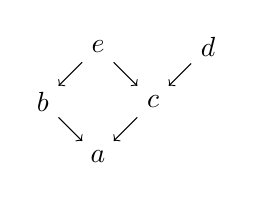
\begin{tikzpicture}[scale=0.7]
	\node (a) at (0,0) {$a$};
	\node (b) at (-1,1) {$b$};
	\node (c) at (1,1) {$c$};
	\node (d) at (2,2) {$d$};
	\node (e) at (0,2) {$e$};
	\draw [->](b) -- (a);
	\draw [->](c) -- (a);
	\draw [->](d) -- (c);
	\draw [->] (e) -- (b);
	\draw [->] (e) -- (c);
\end{tikzpicture}	
\end{center}

A poset can be abstractly represented by a directed graph, which consists of nodes which are connected by arrows. For example, the above graph represents a poset, in which nodes correspond to elements of the poset and arrows tell us how to compare the elements. In particular, an element $x$ is greater than $y$ when there is a directed sequence of arrows from $x$ to $y$.
For example, $c<e$ because of the arrow $e\to c$, and $a<d$ because of $d\to c\to a$. At the same time, $b$ and $c$ are incomparable because there's no arrow between then, as well as $b$ and $d$ are incomparable, etc.

The object of interest to us is called \Emph{affine posets}. They are, loosely speaking, periodic infinite posets --- a poset with infinitely many elements such that the patterns of the arrows are periodic.\footnote{It's worth noting here that, there are many ways to present a permutation, and one of them is using a poset. When the permutation is affine, its poset presentation is indeed an affine poset. This is actually one of the motivations behind the definition of affine posets.} 
%The combinatorics as well as possible algebraic application of affine posets are still open. 

\subsection*{My Result.} In 1950, Dilworth \cite{dilworth1950decomposition} proved a famous decomposition theorem for posets, now known as the \emph{Dilworth's theorem}. Dilworth's theorem studies the minimal way to decompose a poset in to totally ordered sets (called \emph{chains}). In the above example, the poset can be decomposed into two chains: $e\to b$ and $d\to c\to a$, using the smallest number of chains. More specifically, Dilworth's theorem says that the minimal number of chains that we need to decompose a poset equals to the maximal cardinality of a pair-wise incomparable subset of the poset. For example, in the above poset, a maximal pairwise incomparable subset is $\{b,c\}$, having two elements. Dilworth's theorem is directly related the \emph{min-cut max-flow} problem in network theory, and has many other implications in lattice theory and network flows.

In a work-in-progress with my advisor P. Pylyavskyy \cite{PZ}, we proved an analogue of Dilworth's theorem for affine posets. Our \Emph{affine Dilworth's theorem} is also related to certain problems in network theory. In particular, our theorem implies, as a corollary, a 2007 theorem of Bessy and Thomass\'{e} \cite{bessy2007} about the minimal way to cover a network by circuits, which was first conjectured by Gallai in 1963 and remained open for nearly 50 years.


\subsection{Future Plans}I plan to pursue in my thesis research several directions under this line of research, which I will summarize in below.
\subsection*{Affine Greene-Kleitman Correspondence}
An important generalization of Dilworth's theorem is called the \emph{Greene--Kleitman correspondence}, which associates to each poset a ``Young diagram"\footnote{Young diagrams are important ``pictures" which carries a lot of information about the abstract algebras and groups.} Right now, we have a conjectural \Emph{affine Greene-Kleitman correspondence} that we are working towards a proof. 

\subsection*{Affine Permutations and Flag Manifolds} A \emph{flag manifold} is, loosely speaking, a sequence of nested vector spaces.
They are important objects in algebraic geometry and are related to Hilbert's 15th problem. Despite being sophisticated geometric objects, certain aspects of flag manifolds can be understood by combinatorial means. For a pair of two flag manifolds, their ``relative position" is given by a permutation. Moreover, given two flag manifolds, one can use the above-mentioned Greene-Kleitman correspondence to find their relative position. And of course, there should be an affine version of the story.

A flag manifold can also be represented using a matrix, then \emph{affine flag manifolds} can be defined in an analogous way where the representing matrix is an infinite-periodic matrix. Affine flag manifolds are also important in algebraic geometry and Lie theory, but are much more complicated and less understood. There is also a notion of relative position, which is given by an affine permutation. And it remains an open question how to find the relative position of given two affine flag manifolds. Since GK correspondence is proved to be useful in the non-affine setting, we hope that, after proving our conjectural affine GK correspondence, it can be used to give an answer to this question.

\subsection*{Jordan Forms of Infinite-Periodic Matrices} In linear algebra, it is very important to find the \emph{Jordan canonical form} of nilpotent (i.e. upper-triangular) matrices\footnote{A matrix $M$ is nilpotent if multiplying by itself a certain times gives the zero matrix, i.e. $M^k=0$ for some $k$.}. As another application, this can be done using the GK correspondence. 
The affine version of matrices are infinite-periodic matrices, which has a fancier name called \emph{loop groups}. To our knowledge, not much is know about nilpotent elements in loop groups, and we hope to make some progress along this direction.

\subsection*{Possible Connection to Cluster Algebras} Matrices and Flag manifolds are known to have cluster algebra structures. However, the cluster algebra attached to loop groups and affine flag manifold is unknown, though is believed by the experts to exist. In the future, as a more far-reaching goal, I hope to be able make some progress on this question by combining my knowledge in these two different topics.


%\section{Models from Statistical Physics and Special Functions.}In this last section I will summarize the third of my research interests, which is less primary comparing to the previous two.
%
%Statistical physicists created certain \emph{lattice models} to study the behavior of microscopic systems. Loosely speaking, a lattice model is a square grid graph, where we can put certain decorations (usually arrows) on the graph. A lattice model has finitely many ways to decorate, and each way of decoration represents a physical \emph{state} of the system. We can assign a number to each state, called the ``Boltzmann weight'', which is essentially the ``likeliness" of a physical state appearing in the nature. The ``fugacity" of a model is the sum of Boltzmann weights of all possible states, and then the probability of a state can be calculated by taking the ratio of its Boltzmann weight over the fugacity.
%
%Miraculously, these physical models are also natural in mathematics. Physicists would assign real numbers to the states of model, but if we replace these numbers (Boltzmann weights) with special choice of variables, then the fugacity of the model will no longer be a very large number, but instead, certain \emph{special functions} in mathematics. Examples of such special functions are the \emph{Schubert polynomials} and \emph{Schur symmetric polynomials} (special cases of Schubert polynomials). Under such constructions, the \emph{Yang-Baxter equations} of the lattice model becomes very useful in analyzing the resulting special functions from the lattice model. 
%My contribution in this area is a novel lattice model \cite{curran2021lattice} that give rise to LLT polynomials which are quantum deformations of products of Schur polynomials.
%
%The major problem in modern Schubert calculus\footnote{An area of enumerative geometry inspired by Hilbert's 15th problem.} is to calculate the product of two Schubert polynomials. Schur polynomials are special cases of Schubert polynomials. And in the special case of multiplying two Schur polynomials, a formula was given in the seminal work of Allen Knutson and Terence Tao \cite{knutson1999honeycomb}. Recently, the Knutson--Tao formula has been re-derived by Zinn-Justin \cite{zinn2008littlewood} using method from lattice models. Together with A. Hardt and D. Huang, we are planning to work on a project trying to incorporate the lattice model methods (following Zinn-Justin) to make a further progress on this problem --- calculating the product a Schubert polynomial and a Schur polynomial.
\nocite{curran2021lattice}



\bibliographystyle{plain}
\bibliography{RS.bib}
\end{document}